\documentclass[preprint,12pt]{elsarticle}
\usepackage{amsmath,amssymb,booktabs,graphicx}
\usepackage{hyperref}
\hypersetup{hidelinks}
\usepackage{microtype}
\emergencystretch=2em
\journal{Journal of Computational Science}

\newcommand{\mlsl}{\textnormal{MLSL}}
\newcommand{\dfsc}{\textnormal{DFSC}}

\begin{document}
\begin{frontmatter}
\title{A Reliability Protocol for Differentiable Scientific-Computing Primitives in Scientific Machine Learning}
\author[mech]{Ning Hu\corref{cor1}}
\ead{huning@hdu.edu.cn}
\author[cs]{Haitao Duan}
\ead{25050509@hdu.edu.cn}
\author[math]{Shuqun Li}
\ead{Shuqun.Li24@student.xjtlu.edu.cn}
\author[ucsc]{Chuyang Hu}
\ead{chu207@ucsc.edu}
\address[mech]{School of Mechanical Engineering, Hangzhou Dianzi University, Hangzhou, China}
\address[cs]{School of Computer Science, Hangzhou Dianzi University, Hangzhou, China}
\address[math]{School of Mathematics and Physics, Xi'an Jiaotong--Liverpool University, Suzhou, China}
\address[ucsc]{Department of Computer Science and Engineering, University of California, Santa Cruz, CA 95064, USA}
\cortext[cor1]{Corresponding author. ORCID: Ning Hu 0000-0002-2718-0385; Haitao Duan 0009-0006-4611-8639; Shuqun Li 0009-0007-1787-685X; Chuyang Hu 0009-0007-9255-018X.}

\begin{abstract}
Differentiable scientific-computing primitives are increasingly used as structured components in scientific machine learning (SciML), but their numerical value accuracy, parameter gradients, calibration behavior, and module-level reuse are rarely evaluated under one reproducible contract. We present a backend-independent reliability protocol for a batched differentiable map $y=P(x;\theta)$. The protocol requires a declared domain, reference evaluator, value and gradient checks, parameter calibration, module reuse, out-of-distribution (OOD) and long-horizon tests, and device-aware profiling. We instantiate the protocol with four backends: a Mittag--Leffler spectral layer (\mlsl), a matrix-exponential action, a fixed-step linear RK4 step, and a nonlinear Logistic-equation RK4 step. The evidence is intentionally backend-specific. The matrix-exponential and RK4 backends pass value, gradient, calibration, module-reuse, OOD, and long-horizon gates on their declared low-dimensional domains. A common neural OOD task shows that primitive composition can improve the Logistic backend but does not uniformly improve the matrix backend. This negative result is part of the protocol's purpose: it separates reliable differentiability from task-level predictive benefit. The resulting open implementation provides a registry and auditable JSON reports for reusable SciML components, while its current scope remains controlled benchmark domains rather than a universal solver library.
\end{abstract}

\begin{keyword}
scientific machine learning \sep differentiable primitive \sep automatic differentiation \sep numerical reliability \sep parameter calibration \sep reproducibility
\end{keyword}
\end{frontmatter}

\section{Introduction}
SciML models increasingly combine learned modules with numerical maps such as propagators, matrix-function actions, integration steps, and structured residual blocks. Automatic differentiation supplies derivatives of numerical programs, but the existence of an autodiff trace is not a numerical error guarantee \citep{baydin2018autodiff}. A primitive can therefore be differentiable in a software sense while still producing inaccurate values, unstable parameter sensitivities, or unreliable calibration.

This paper studies the missing evaluation contract rather than proposing a new universal solver. We define a portable protocol that makes four questions explicit: (i) is the value accurate on a declared domain, (ii) are parameter gradients numerically credible, (iii) can parameters be calibrated from observations, and (iv) can the primitive be reused inside neural and physics-informed modules? OOD, long-horizon, batch/device, and finite-gradient checks are treated as additional reliability gates.

Our contributions are: (1) a backend-independent primitive contract and normalized audit schema; (2) a public Python implementation with registry, profile, and audit APIs; (3) cross-backend evidence covering a fractional propagator case study and three non-fractional controls; and (4) a matched module-level OOD test that records both positive and negative task outcomes. The contribution is methodological and reproducibility-oriented: the protocol is a way to compare and qualify primitives, not a claim that one backend dominates all others.

\section{Related Work and Positioning}
The protocol is complementary to differentiable programming systems such as DiffTaichi \citep{hu2020difftaichi}, scientific machine learning formulations such as universal differential equations \citep{rackauckas2020universal}, and neural operators that learn maps between function spaces \citep{kovachki2023neuraloperator}. Fractional propagation also has a mature numerical literature, including discretized fractional calculus \citep{lubich1986discretized}, Mittag--Leffler evaluation \citep{garrappa2015mittag,gorenflo2014mittag}, and fractional Laplacian definitions \citep{lischke2020fractional}. Those areas provide algorithms and model classes; the present work specifies evidence required before a numerical component is treated as a reusable SciML primitive.

\section{Primitive Contract}
Each backend exposes a batched map
\begin{equation}
    y=P(x;\theta),
\end{equation}
with an explicit input and parameter domain, output shape, dtype policy, device policy, and reference evaluator. The protocol does not require every primitive to share the same mathematics. It requires the evaluation record to preserve the domain on which each claim is valid.

\subsection{Reliability dimensions}
Value fidelity is measured against a declared reference using absolute and relative errors and finite-value rates. Differentiability is assessed using finite-gradient rates and directional derivative discrepancies. Calibration uses noisy observations and reports parameter error, convergence behavior, seed variation, and a matched non-gradient baseline where available. Module reuse evaluates at least two compositions, including a neural module and a batched operator or physics objective. OOD, long-horizon, and batch/device tests expose boundary behavior rather than collapsing it into one score.

\section{Implementation}
The implementation is provided in the \texttt{P4/dfsc\_protocol} package. \texttt{audit\_value\_and\_gradient} checks finite outputs and gradients; \texttt{audit\_batch\_and\_device} checks batched execution and device locality; the registry records dimension-level gate states and scope limits; and the profile schema stores latency, throughput, memory, dtype, and device metadata. Reports are JSON and are generated from experiment outputs rather than manually transcribed tables.

\begin{figure}[t]
\centering
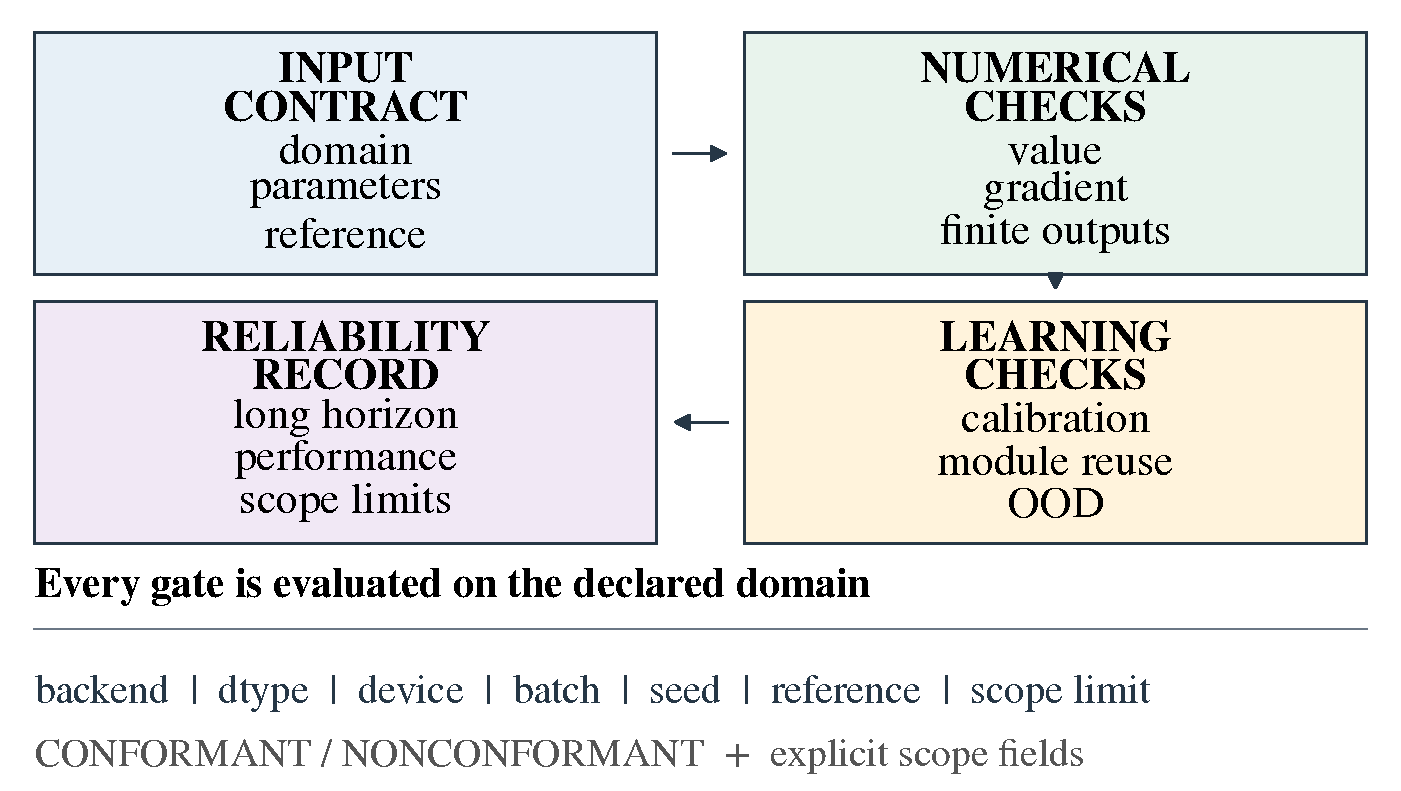
\includegraphics[width=0.98\linewidth]{figures/fig_protocol.pdf}
\caption{The proposed primitive reliability workflow. Each gate is evaluated on a declared domain and recorded with implementation metadata and scope limits.}
\label{fig:protocol}
\end{figure}

\section{Experimental Design}
The current evaluation uses controlled low-dimensional problems so that reference values and directional derivatives are auditable. The four backends are \mlsl, matrix-exponential action, fixed-step linear RK4, and Logistic RK4. The non-\mlsl backends are substantive controls for testing whether the protocol survives different numerical structures. All reported multi-seed experiments use five seeds unless otherwise stated. The common neural OOD task uses three seeds, 512 training tasks, 256 test tasks, two target times ($1.0$ and $1.5$), and two observation-noise levels ($0.003$ and $0.01$) on an RTX 5070 Laptop GPU.

\section{Results}
\subsection{Cross-primitive gate coverage}
The registry contains four backend records and six required dimensions: value, gradient, calibration, module reuse, OOD, and long horizon. We additionally reran the MLSL backend through the P1 public factory API using the stable hybrid configuration. On the declared one-dimensional Dirichlet, negative-real spectral regime, the maximum relative value error against an 80-digit reference series was $1.32\times10^{-12}$; alpha and beta gradient errors against central differences were $2.22\times10^{-9}$ and $5.00\times10^{-10}$. Joint calibration recovered $(\alpha,\beta)=(0.78003,1.80007)$ from $(0.90,2.10)$ initialization. The MLSL row therefore passes all six protocol gates, while retaining its stated scope limits. All four records have status \texttt{pass\_with\_scope\_limits}.

\begin{table}[t]
\centering
\caption{Representative multi-seed reliability results. Values are backend-specific and are not pooled into an accuracy ranking.}
\resizebox{\linewidth}{!}{%
\begin{tabular}{lccc}
\toprule
Backend & OOD value error & Directional gradient error & Calibration L1 error\\
\midrule
Matrix exponential action & $4.27\times10^{-15}$ long-horizon max & $3.79\times10^{-11}$ & $3.11\times10^{-4}$\\
Linear RK4 step & $1.67\times10^{-3}$ OOD max & $2.48\times10^{-10}$ & $6.71\times10^{-4}$\\
Logistic RK4 step & $7.52\times10^{-6}$ OOD max & $4.41\times10^{-11}$ & $2.60\times10^{-2}\pm2.46\times10^{-2}$\\
\bottomrule
\end{tabular}%
}
\end{table}

The matrix action maintains a mean long-horizon maximum absolute error of $4.27\times10^{-15}$ over five seeds and time points from $0.02$ to $12$. Linear RK4 has mean OOD maximum absolute error $1.67\times10^{-3}$ over step sizes $0.41$--$0.80$; its long-horizon errors at $t=5$ are $1.48\times10^{-9}$ for step size $0.05$ and $4.23\times10^{-7}$ for $0.20$. Logistic RK4 has mean OOD maximum absolute error $7.52\times10^{-6}$ over step sizes $0.26$--$0.50$, but its calibration error is materially larger. These results demonstrate why a protocol must preserve backend-specific error budgets.

\subsection{Public-data transfer}
We additionally evaluated the structured primitive on two provenance-aware public datasets. For the GeoTES pilot-scale thermocouple histories (Zenodo DOI \href{https://doi.org/10.5281/zenodo.18979098}{10.5281/zenodo.18979098}), the first measured heating/cooling cycle was used for identification and the second cycle for transfer. Across three seeds, the DFSC-plus-residual model obtained a cycle-2 relative error of $0.3619\pm0.0085$, compared with $0.3632\pm0.0071$ for a pure MLP, using 750 rather than 1251 parameters. For the heated-steam temperature profiles (Zenodo DOI \href{https://doi.org/10.5281/zenodo.15064388}{10.5281/zenodo.15064388}), held-out-condition RMSE was $43.33\pm0.56$ K for direct DFSC, $16.03\pm0.14$ K for the hybrid, and $13.25\pm1.45$ K for the pure MLP. The latter result is retained as a negative task-level finding: a reliable primitive does not imply unconditional predictive superiority. These experiments support real-data transfer and scope diagnosis rather than universal physical identification.

To separate observation density from extrapolation-horizon effects, we also repeated the GeoTES experiment with
uniform subsampling over the full first cycle while retaining the second cycle as a fixed holdout. At 40\% coverage,
the hybrid reached $0.3607\pm0.0082$ versus $0.3657\pm0.0084$ for the pure MLP, again with 750 versus 1251
parameters. The hybrid did not improve the MLP at 20\%, 60\%, or 100\% coverage. We therefore interpret the result
as a conditional benefit in a moderate-data regime, rather than as evidence of monotone few-shot superiority.

\subsection{Module-level OOD evidence}
In the common neural task, the Logistic primitive improves OOD RMSE relative to a pure MLP at both target times and both noise levels: for example, at $t=1.5$ and noise $0.003$, the primitive gives $0.2340\pm0.0323$ versus $0.2713\pm0.0096$ for the MLP. The matrix primitive does not improve this task: at the same setting it gives $0.1998\pm0.0272$ versus $0.1638\pm0.0097$. Training with a primitive is also slower in this implementation. The result is therefore a task-conditional benefit, not a universal predictive advantage.

\begin{figure}[t]
\centering
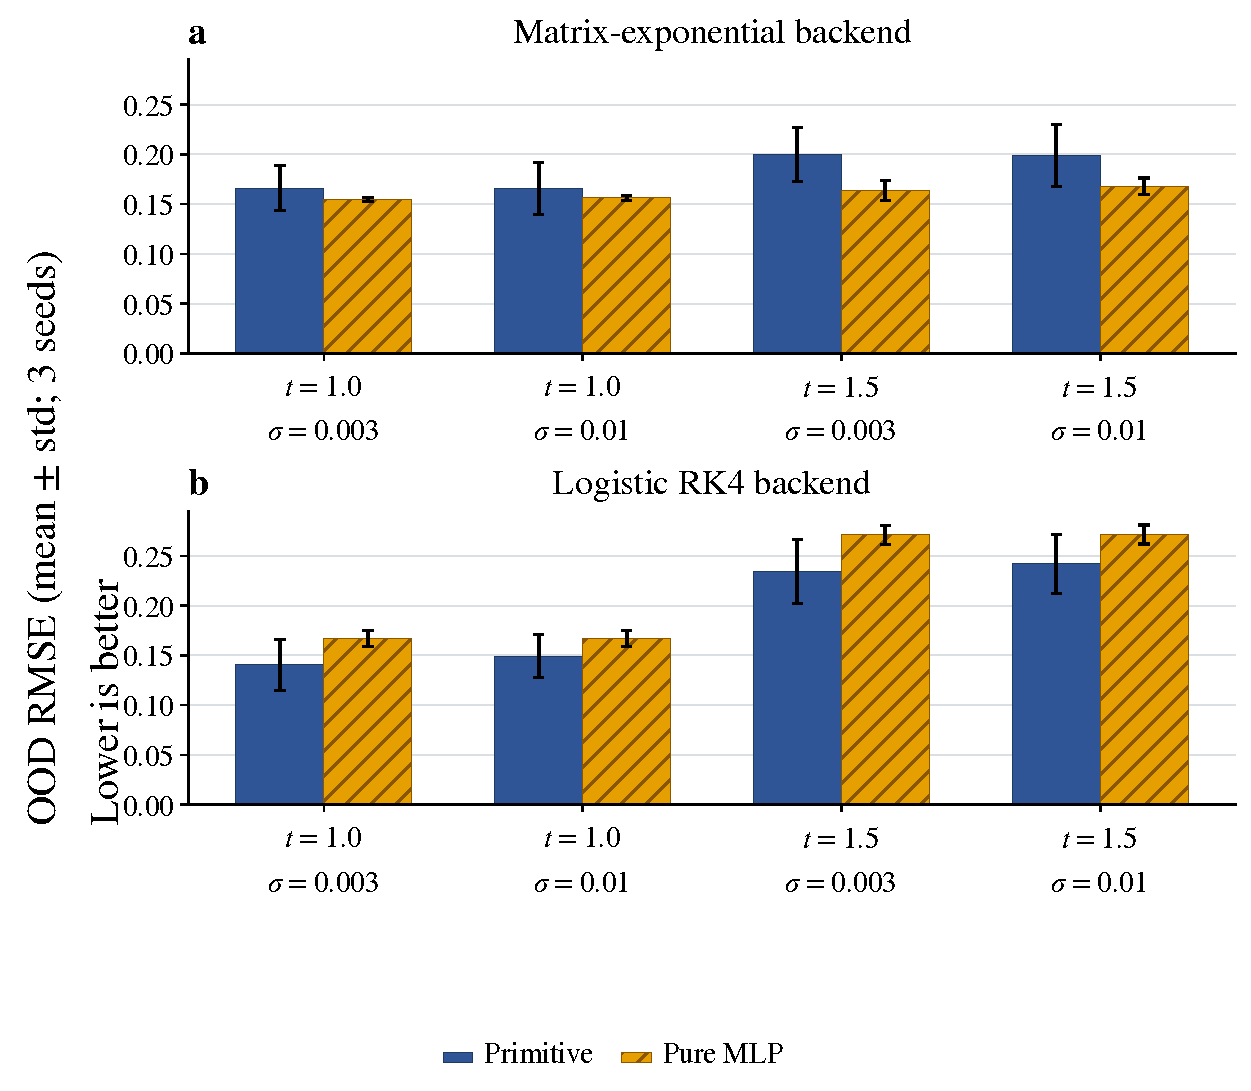
\includegraphics[width=0.98\linewidth]{figures/fig_common_ood.pdf}
\caption{Common module-level OOD task. The Logistic primitive improves OOD RMSE in the tested settings, whereas the matrix primitive does not uniformly improve the pure MLP control. Numerical means and standard deviations are reported in the source JSON.}
\label{fig:common-ood}
\end{figure}

\subsection{Batch and GPU profile}
On the RTX 5070 Laptop GPU, all tested backends produced finite outputs for batch sizes 1, 64, 256, and 1024 in float64. Throughput increased with batch size, but the measurements are implementation profiles rather than a cross-domain speed ranking. The profile records warmup count, synchronized timing, peak memory, dtype, and output shape so that future backends can be compared under the same reporting contract.

\begin{figure}[t]
\centering
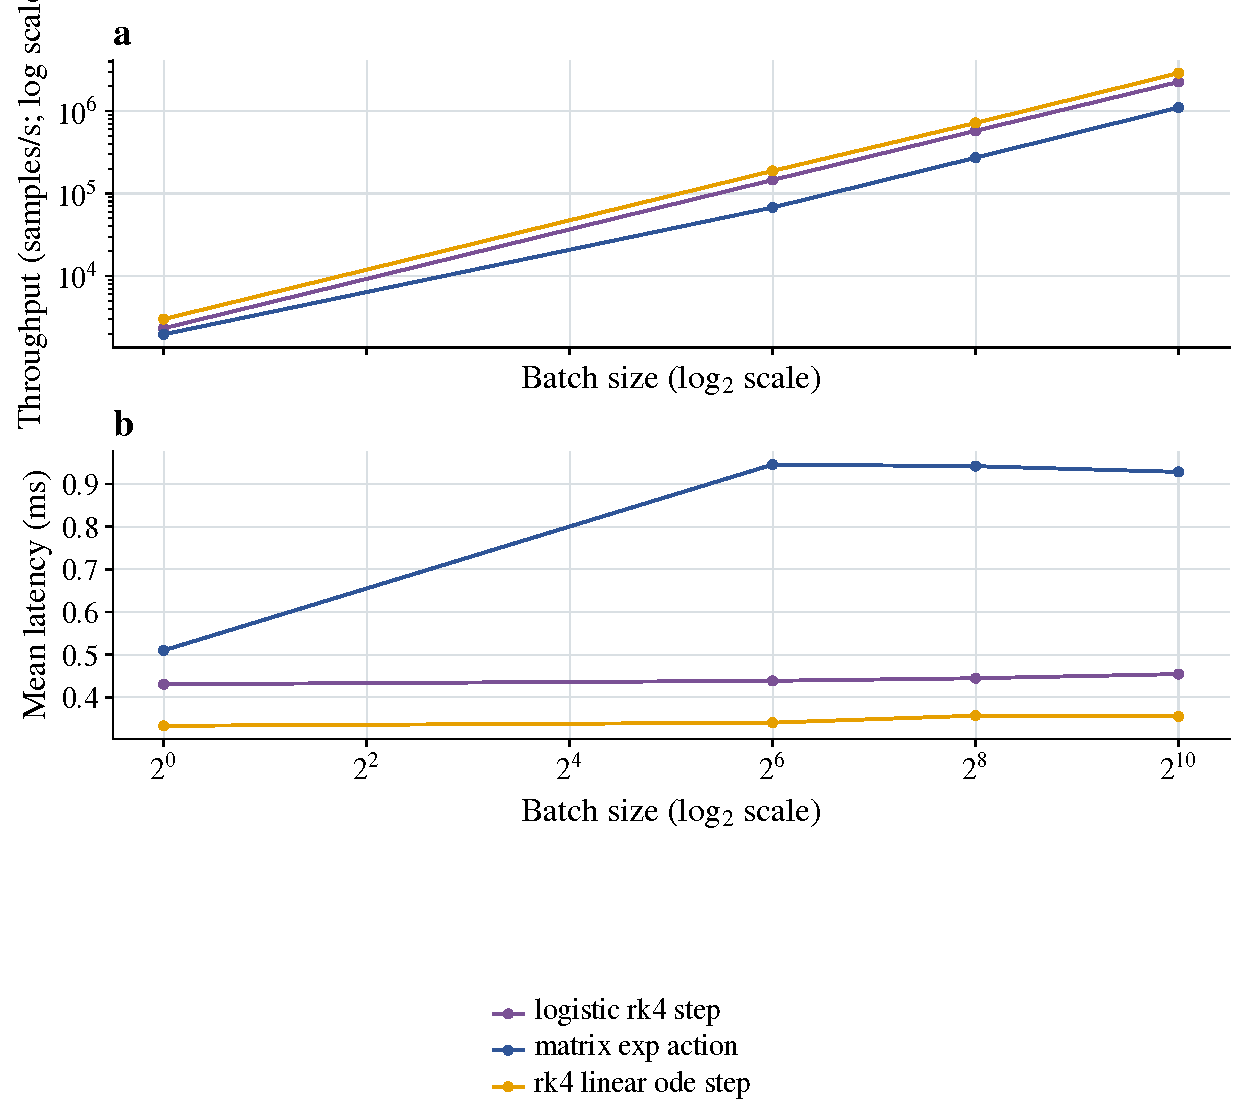
\includegraphics[width=0.86\linewidth]{figures/fig_gpu_profile.pdf}
\caption{Batch throughput profile on the RTX 5070 Laptop GPU. The curves are implementation profiles for the declared low-dimensional backends, not a cross-domain speed ranking.}
\label{fig:gpu-profile}
\end{figure}

\section{Discussion and Scope}
The main evidence supports protocol reuse, not universal solver superiority. The current study combines controlled low-dimensional domains with two public-data transfer tests and PyTorch execution. It does not validate variable-order or distributed-order fractional operators, complex geometries, unstructured meshes, JAX or Julia backends, or universal physical identification. These limitations define the next validation targets and prevent the protocol from being described as a complete fractional solver library.

\section{Reproducibility and Availability}
Experiment scripts, JSON results, registry/profile schemas, package tests, and the paper-data builder are kept under \texttt{P4} in the public repository \href{https://github.com/hzhooning-art/DFSC}{github.com/hzhooning-art/DFSC}. The manuscript tables should be regenerated with \texttt{python paper/build\_paper\_data.py}. The hosted CPU workflow passed on GitHub Actions for the tested software commit \texttt{20fab75} (workflow run \href{https://github.com/hzhooning-art/DFSC/actions/runs/31581391771}{31581391771}). The current local test suite also passes. The repository records the implementation and audit artifacts; external reproduction remains a recommended independent check rather than a claimed completed result.

\section{Conclusion}
We introduced and tested a reliability protocol for differentiable scientific-computing primitives in SciML. By separating value fidelity, gradient credibility, calibration, reuse, OOD behavior, long-horizon stability, and hardware profiling, the protocol makes claims auditable and preserves negative results. The current evidence supports a reusable evaluation and software interface on declared domains, with \mlsl as the motivating fractional case study. Broader numerical domains and independent external validation are required before making stronger ecosystem-wide claims.

\section*{Data and Code Availability}
The code and generated JSON reports are organized in the P4 project directory. A public release and DOI should be cited only after the corresponding release has been created and verified.

\section*{CRediT authorship contribution statement}
Ning Hu: Conceptualization, Methodology, Software, Validation, Formal analysis, Investigation, Data curation, Visualization, Writing - original draft, Writing - review and editing. Haitao Duan: Methodology, Software, Validation, Investigation, Writing - review and editing. Shuqun Li: Validation, Investigation, Writing - review and editing. Chuyang Hu: Validation, Investigation, Writing - review and editing.

\section*{Declaration of competing interest}
The authors declare that they have no known competing financial interests or personal relationships that could have appeared to influence the work reported in this paper.

\section*{Declaration of Generative AI and AI-Assisted Technologies}
During preparation of this manuscript, the authors used AI-assisted tools for language editing, organization of manuscript drafts, consistency checks, and code/documentation review. The authors reviewed, edited, and verified the resulting text, numerical claims, references, and software statements, and take full responsibility for the final content. AI tools were not used to generate or fabricate experimental data.

\bibliographystyle{elsarticle-num}
\bibliography{references}

\end{document}
